% !TEX root=/home/tavant/these/manuscript/src/manuscript.tex

% \FloatBarrier

\section{Comparison of the sheath model with PIC simulations} \label{subsec-picandmodel}

  % \begin{figure}[hbtp]
  %   \centering
  %   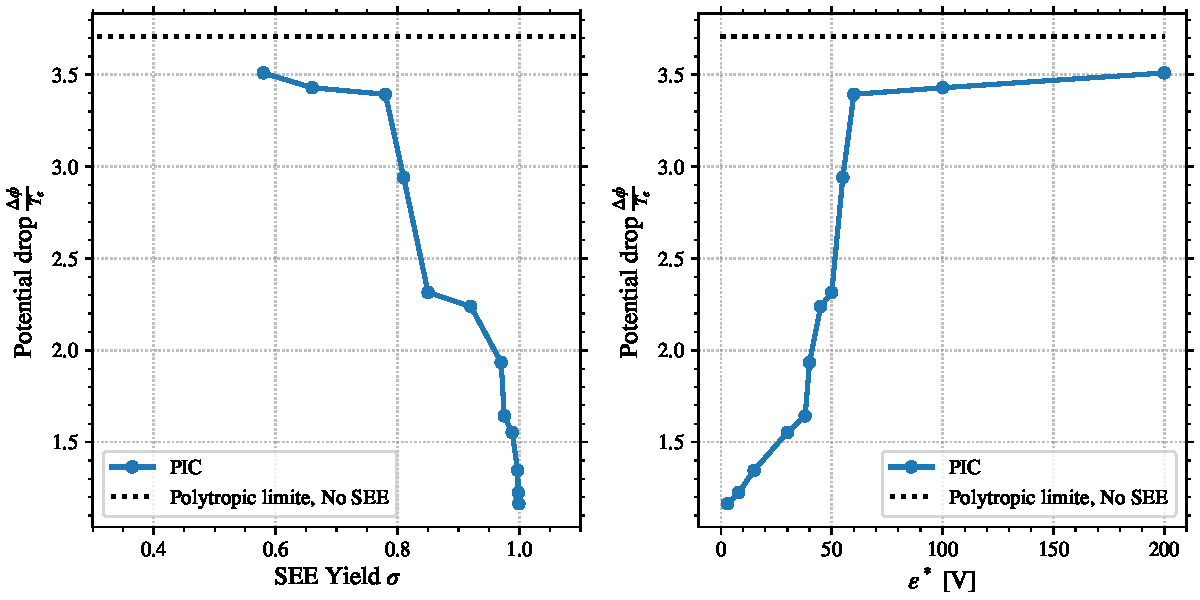
\includegraphics[width=\textwidth]{dphi_polytropic_noSEE}
  %   \caption{PIC simulation results (with SEE) compared to the polytropic limit without SEE.}
  %   \label{fig-polytropic_pic_noSEE}
  % \end{figure}
  % 
  % \begin{figure}[hbtp]
  %   \centering
  %   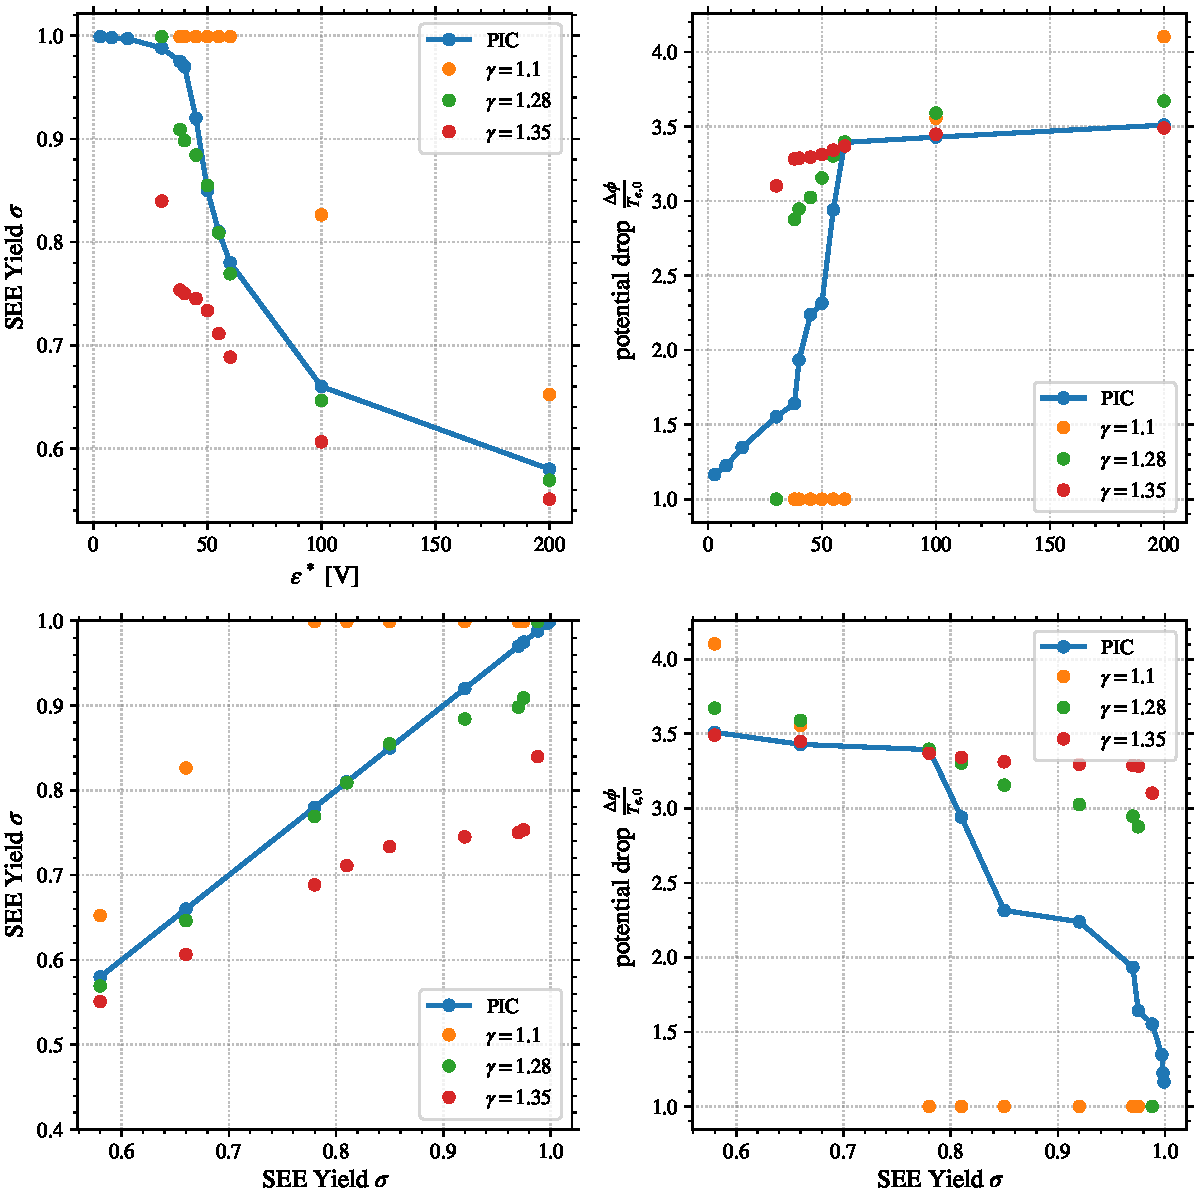
\includegraphics[width=\textwidth]{Summary_polytropic_SEE.pdf}
  %   \caption{Comparison of the PIC simulation results with the polytropic model with SEE.}
  %   \label{fig-polytropic_see_summary}
  % \end{figure}

  We compare in this section the characteristics of the plasma wall interaction observed in the \ac{PIC} simulations with the fluid model developed in \cref{sec-fluid_poly_see}.
  We first compare the mean values using in the parametric study over the crossover energy $\crover$, then we investigate the oscillation of ragime {\bf II}.

  \subsection{Parametric study of the modified sheath model} \label{subsec-param_sheath_see}

    The variables of interest are the averaged electron emission rate $\rate$ and the plasma potential drop to the wall.
    The only input of the model is the electron mean temperature in the bulk $\Teb$ as well as the polytropic index $\gamma$.
    As seen in \cref{sec-PIC_poly}, the polytropic index of the electron population is measured in the \ac{PIC} simulation to $\gamma=1.35$.
    However, the electrons going toward the wall present a different index, measured from the bulk \ac{EVDF} to $\gamma=1.28$.
    These two values will be compared.

    Using the mean electron temperature measured in the simulation, we first compute the plasma potential drop $\dphi$ by solving \cref{eq-costseepoly} with $\gamma=1.35$.
    As showed in \cref{fig-rso_crit_see}, up to three solutions are possible.
    The emission rate $\rate$ is then computed using \cref{eq-seemaxw_Tew}, using the two values for $\gamma$.
    As discussed previously, the rate is limited to $\ratecr=0.982$ to take into account the \ac{SCL} regime.

    The results are shown in \Cref{fig-Poly_model_vs_pic}.
    The plasma potential drop computed is increased by $\Teb/2$ corresponding to the pre-sheath drop to better match the plasma potential measured in the simulations.
    \improvement{The Bhom criterion is slightly modified with the polytropic model, so it should not exactly be $\Teb/2$. however, it matches to well here that I do not really want to change !}

    \begin{figure}[hbtp]
      \centering
      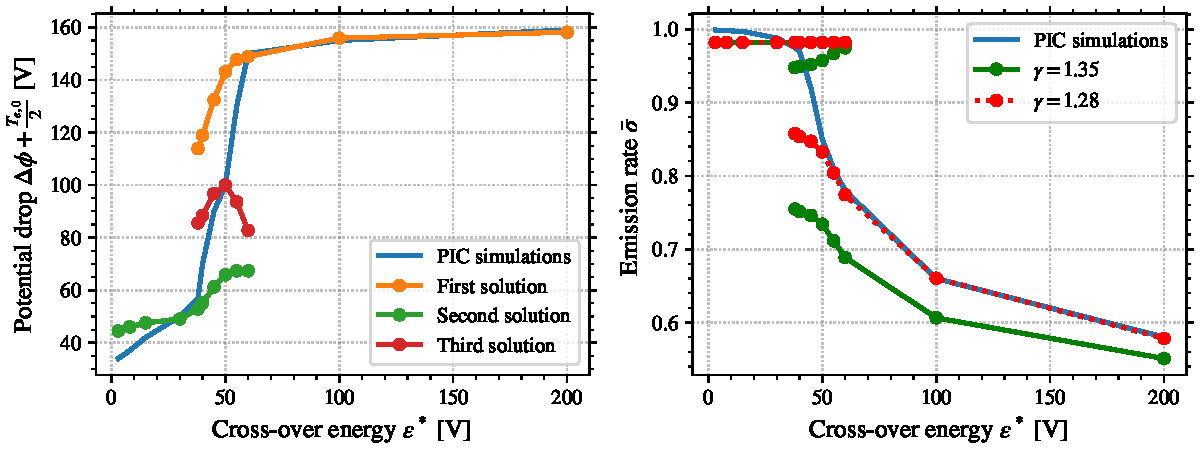
\includegraphics[width=\textwidth]{Poly_model_vs_pic}
      \caption{Comparison of the PIC simulations and the sheath model for the plasma potential drop from the center to the wall and the electron emission yield. }
      \label{fig-Poly_model_vs_pic}
    \end{figure}

    Concerning $\dphi$, we can see that the sheath model combining the polytropic state law and the electron emission is in good agreement with the \ac{PIC} simulations.
    We can see that the region where the three solutions coexist corresponds well with the regime {\bf II}.

    For the emission rate $\rate$, we observe that the value $\gamma=1.35$ under estimates $\rate$ compared to the values of the \ac{PIC} simulations.
    On the other hand, $\gamma=1.28$ is in very good agreement.

    Interestingly, at the saturation the mean electron emission rate in the \ac{PIC} simulation is greater than the critical value $\ratecr$.
    \inlinenote{ As $\rate$ is better with $\gamma=1.28$, we should use both values in \cref{eq-costseepoly}. However, this increases the complexity the equations and the model, and add 1 more free parameters (they would be 2 values for $\gamma$ now). I can say that only in the discussion maybe ? }
    
  \subsection{Sheath oscillation of regime {\bf II}} \label{subsec-pic_scheath_RSO}
  
    The regime {\bf II}, presents oscillations between two meta-stable states, one with a low emissivity and the other with a high emissivity.
    \Cref{fig-long_time} shows the temporal evolution of the electron temperature and the plasma potential relative to the wall for $\crover=45\,\volt$.
    The electron temperature is computed over the wholme electron population in the simulation.
    Both the radial temperature $\Te_{,R}$ and the total and averaged, temperature $\Te$ are shown.
    The plasma potential $\dphi$ showed is measured at the center of the radial direction of the simulation, averaged over the azimuthal direction.
    
    
    \begin{figure}[hbtp]
      \centering
      \begin{tabular}{c c}
        \subfigure{long_time_dphi}{a}{20,20} &
        \subfigure{long_time_Te}{b}{20,20} \\
      \end{tabular}
      \caption{Temporal evolution of ({\bf a}) the plasma potential $\dphi$ and ({\bf b}) the electron temperature.}
      \label{fig-long_time}
    \end{figure}
    
    We clearly see in \cref{fig-long_time} the quasi-periodic oscillations between the two states.
    We observed that the electron temperature is slightly anisotropic, with the radial temperature smaller than the axial temperature.
    This anisotropy observed was not taken into account the sheath model.
    Hence, we will compare the prediction using only the radial temperature $\Te_{,R}$ and the total, averaged, temperature $\Te$.
    
    \Cref{fig-dphi_te_PIc} shows the potential drop as a function of the electron temperature measured in the \ac{PIC} simulation (same case as \cref{fig-long_time}).
    Is also shown the theoretical solutions obtained with the model of \cref{sec-fluid_poly_see} using a constant polytropic index $\gamma=1.34$ and $\crover=45\,\volt$.
    
    \begin{figure}[hbtp]
      \centering
      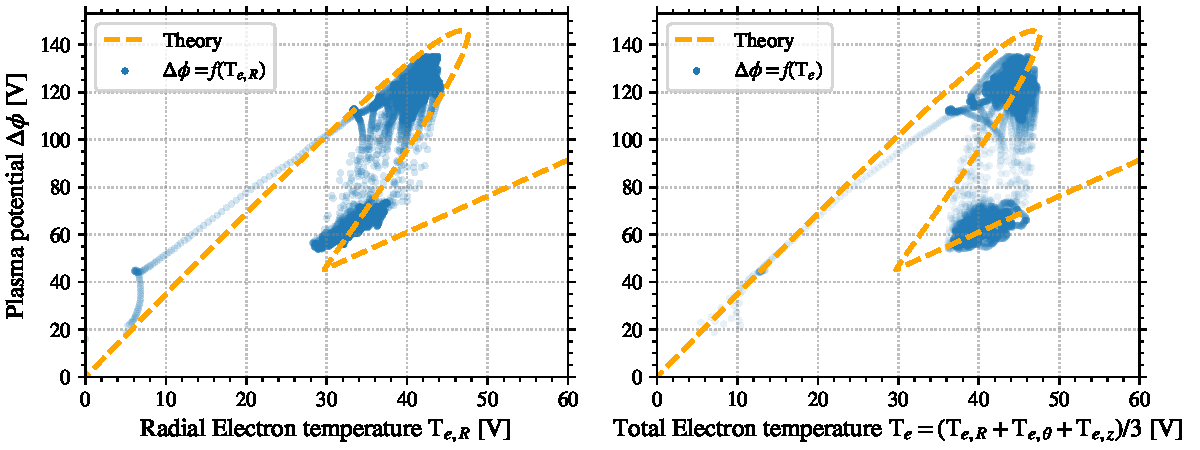
\includegraphics[width=\textwidth]{parametric_PIC_dphi_Te}
      \caption{Plasma potential as a function of (left) the radial electron temperature and (left) the total electron temperature. The blue markers represents the \ac{PIC} results presented in \cref{fig-long_time}, and the orange dashed lines correspond to the theoretical values.}
      \label{fig-dphi_te_PIc}
    \end{figure}
    
    We can see in \cref{fig-dphi_te_PIc} that the sheath characteristics observed in the \ac{PIC}  simulations matches relatively well the theoretically values.
    In particular, we see the cohabitation of the two solutions of $\dphi$ observed for the same electron temperature, which corresponds to the domain of electron temperature for which the sheath model also predicts multiple solutions.
    
